\documentclass[a4paper, 12pt]{report}
\usepackage[top = 2.54cm, bottom = 2.54cm, left = 2.54cm, right = 2.54cm]{geometry}
\usepackage{graphicx}
\usepackage{enumerate}
\usepackage{amsmath}
\usepackage{verbatim}
\usepackage{fancyhdr}
\usepackage{fixltx2e} % Package for subscripting and superscripting... %
\pagestyle{fancy}
\setlength{\parindent}{0pt}
\lhead{}
\rhead{Group D - Phase 2 Report}
\renewcommand{\headrulewidth}{0.3pt}

\title{Influenza Virus Infection Modeling}
\author{A.~Ambuehl -- \texttt{antonietta.ambuehl@dtc.ox.ac.uk} \and J.~Leem -- \texttt{jinwoo.leem@dtc.ox.ac.uk} \and M.~Lucken -- \texttt{malte.lucken@dtc.ox.ac.uk} \and W.~Smith -- \texttt{william.smith@dtc.ox.ac.uk} \and O.~Thomas -- \texttt{owen.thomas@dtc.ox.ac.uk} \\\\
University of Oxford DTC \\
Rex Richards Building \\
South Parks Road\\
\underline{Oxford, OX1 3QZ, United Kingdom}\\
}

\begin{document}
\maketitle

%% STYLISTIC COMMENTS %%
%
% Please format function names in computer modern (>> "\textt{}") and latin (i.e., etc., via, e.g.) in italic (>> "\textit{}")
% Citations take >> "glim~\cite{paper}" to give proper spacing.
% Acronymns (as with any other object) should not be pluralised using an apostrophe. (so ODEs not ODE's)
% Don't use the regular speechmarks, they are not formatted correctly (so ``speech'  not "speech"')
% Strings of references take individual boxes (so \cite{X}~\cite{Y}~\cite{Z} rather than \cite{X,Y,Z})
% MatLab is refered to as ">> MatLab\textsuperscript{\textregistered} "

%%Add these to the Bib

\begin{abstract}
This work is licensed under the Creative Commons Attribution-ShareAlike 3.0 Unported License. To view a copy of this license, visit http://creativecommons.org/licenses/by-sa/3.0/ or send a letter to Creative Commons, 444 Castro Street, Suite 900, Mountain View, California, 94041, USA.
\end{abstract}

\chapter{Background and Aims} %Done by Jin
\section{Biological Problem and Previous Work}

The influenza virus is responsible for considerable public discomfort, and poses the risk of seasonal pandemic and a potentially major health hazard to the elderly or infirm.~\cite{Smith} For the purposes of treating and preventing viral infections, it would be desirable to generate a model which simulates the course of viral infection. Models that study the interplay between immune system components within an individual suffering from viral infection have previously been developed (for a review, see Perelson 2002~\cite{Perelson}), and have the potenital to capture multiple aspects of human epithelial immunology (\textit{e.g.} interaction of cytokines, effector cells, antibodies, virions, \textit{etc.}). 

In particular, a model was devised in 2007 which encompassed many of the factors involved in human-virus immune response ~\cite{Hancioglu}, such as:

\begin{itemize}
\item Antibodies and their affinity toward the circulating virus;
\item Antigen presentation;
\item Production and clearance of the virus, \textit{etc.}.
\end{itemize}

This paper of Hancioglu \textit{et al.} featured a continuum model based on a series of ordinary differential equations (ODEs). The model was used predict changes in the population of healthy and infected cells, and levels of the free virus over the course of infection. \\

In 2013, the results of the model have been reproduced by members of Group G by using a series of Matlab\textsuperscript{\textregistered} and C++ code~\cite{GroupG}. This computational model successfully reproduces cellular and viral dynamics in a hypothetical infection scenario, displaying good fidelity. In addition, the authors provide an open-source implementation of the model in MatLab\textsuperscript{\textregistered}, featuring a graphic user interface (GUI) that enables users to control and systematically parse the model's 27 parameters, as well as facilitating the visualisation of multiple datasets. \\

\section{Identification of areas for extension}

Although the model is designed so that parameters can be tailored to each patient's immune capacity and each virus strain's virulence, it only reflects the natural biological response (\textit{i.e.} the adaptive and innate immune responses) to the virus. Moreover, the model was entirely deterministic: real biological processes tend to involve considerable noise, and several of the processes included in the system are thought to be intrinsically stochastic. Finally, we noted that the mode omitted certain interactions between immune system components.
Our group felt that the model could be extended further by:
\begin{enumerate}
\item Considering the effects of anti-influenza drugs on the cellular and viral dynamics;
\item Converting the coupled ODE representation to include stochastic noise;
\item Including the influence of helper T-cells (T\textsubscript{H} cells), which help to form plasma cells.
\end{enumerate}
In addition, we scrutinised the code of their implementation closely, and investigated ways in which it could be rewritten in a more efficient manner. Ultimately, these extensions culminated to a new model as shown in Figure~\ref{newmodel}:

\begin{figure}[htb]
\label{newmodel}
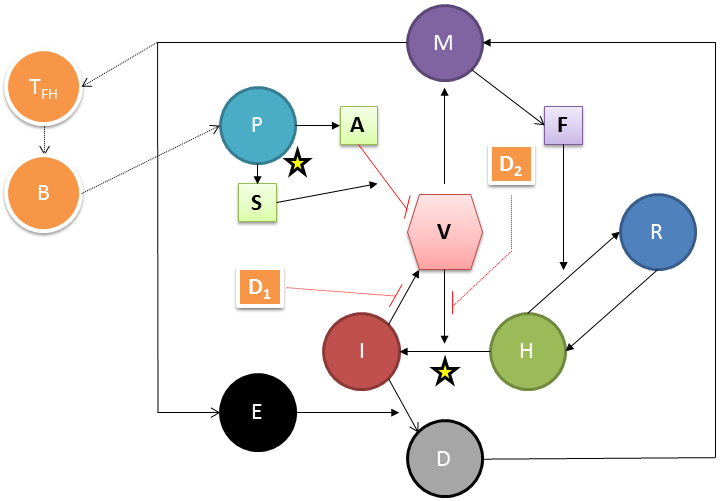
\includegraphics[width = 150mm]{Diagram.png}
\caption{Each of the relevant compartments, as per the original model, are labelled in their respective abbreviations (\emph{e.g.} Infected cells are represented by $I$ and antigen presenting cells (APCs) are represented by $M$, \emph{etc.}). Our additions to the model are labelled as orange compartments with dotted lines for their relevant processes. These new additions include: drugs (neuraminidase inhibitors, $D_1$, and amantadine $D_2$), helper T cell:B cell dynamics (T\textsubscript{FH} and B) and introduction of stochasticity (labelled with yellow stars).}
\end{figure}

\chapter{Extension of the Model}
\section{Extension of the Model I -- Modelling Antiviral therapy}

To extend the model, we decided to investigate the effects of adding an antiviral agent to the system. Antivirals are drugs used to control viral infections both therapeutically and prophylactically. They operate by interfering with the virus copying sequence at one or more points in its replication cycle. For example, two common antiviral targets are:
\begin{enumerate}
\item \textbf{Viral M2 proton channels:} Disruption of viral unpackaging in host cytosol \textit{via} the competitive inhibition of the viral M2 proton channel;~\cite{Hu}
\item \textbf{Viral Neuraminidase:} Prevention of viral budding \textit{via} competitive inhibition of the neuraminidases responsible for severing newly-created virus particles from their host cells.\cite{Satoh}  
\end{enumerate}
Instances of antivirals exploiting the above mechanisms include  Amantadine (trade name ``Symmetrel'') and Oseltamivir phosphate (``Tamiflu'').\\
%Tamiflu works by inhibiting the action of the enzyme viral neuraminidase, whose action is necessary to allow newly-created viral particles to detach from their infected hosts.S
%Symmetrel, an older drug, operates by interfering with the action of viral M2 proton channels, preventing virus particles from becoming decoated once they are absorbed into cells by endocytosis.

\subsection{Including Drug Variables in Existing Model}

Kinetic models have previously been used to investigate the influence of an antiviral drug on viral dynamics within infected individuals -- such as the recent work of Smith \textit{et al.}~\cite{Smith} who modelled drug influences in simple kinetic models.
The influence of the 2 drug types was accommodated by changing terms in equations (1), (2) and (3), to redescribe the relationship between the variables $H$ (healthy cells), $I$ (Infected cells) and $V$ (Virus particles):

\begin{itemize}
\item  $\gamma_{HV}VH \rightarrow \gamma_{HV}(1 - \epsilon)VH$ in the case of Amantadinoid drugs;
\item $\gamma_{V}I \rightarrow \gamma_{V}(1 - \epsilon)I $ in the case of Neuroamidinase Inhibitors.
\end{itemize}

%$\epsilon\left(t\right)$
where $\epsilon$ represents the drug's efficacy. In their paper, Smith \textit{et al.} assumed a drug concentration, and therefore an $\epsilon$ value, that was constant with respect to time -- generally, this assumption would be inappropriate, as the amount of drug present in bodily tissues varies as it is degraded and excreted. We sought to extend the work from reference~\cite{Smith} by combining a more realistic, temporal drug model with the extended dynamic model of group G.\cite{GroupG}

\begin{figure}[htb]
\begin{centering}
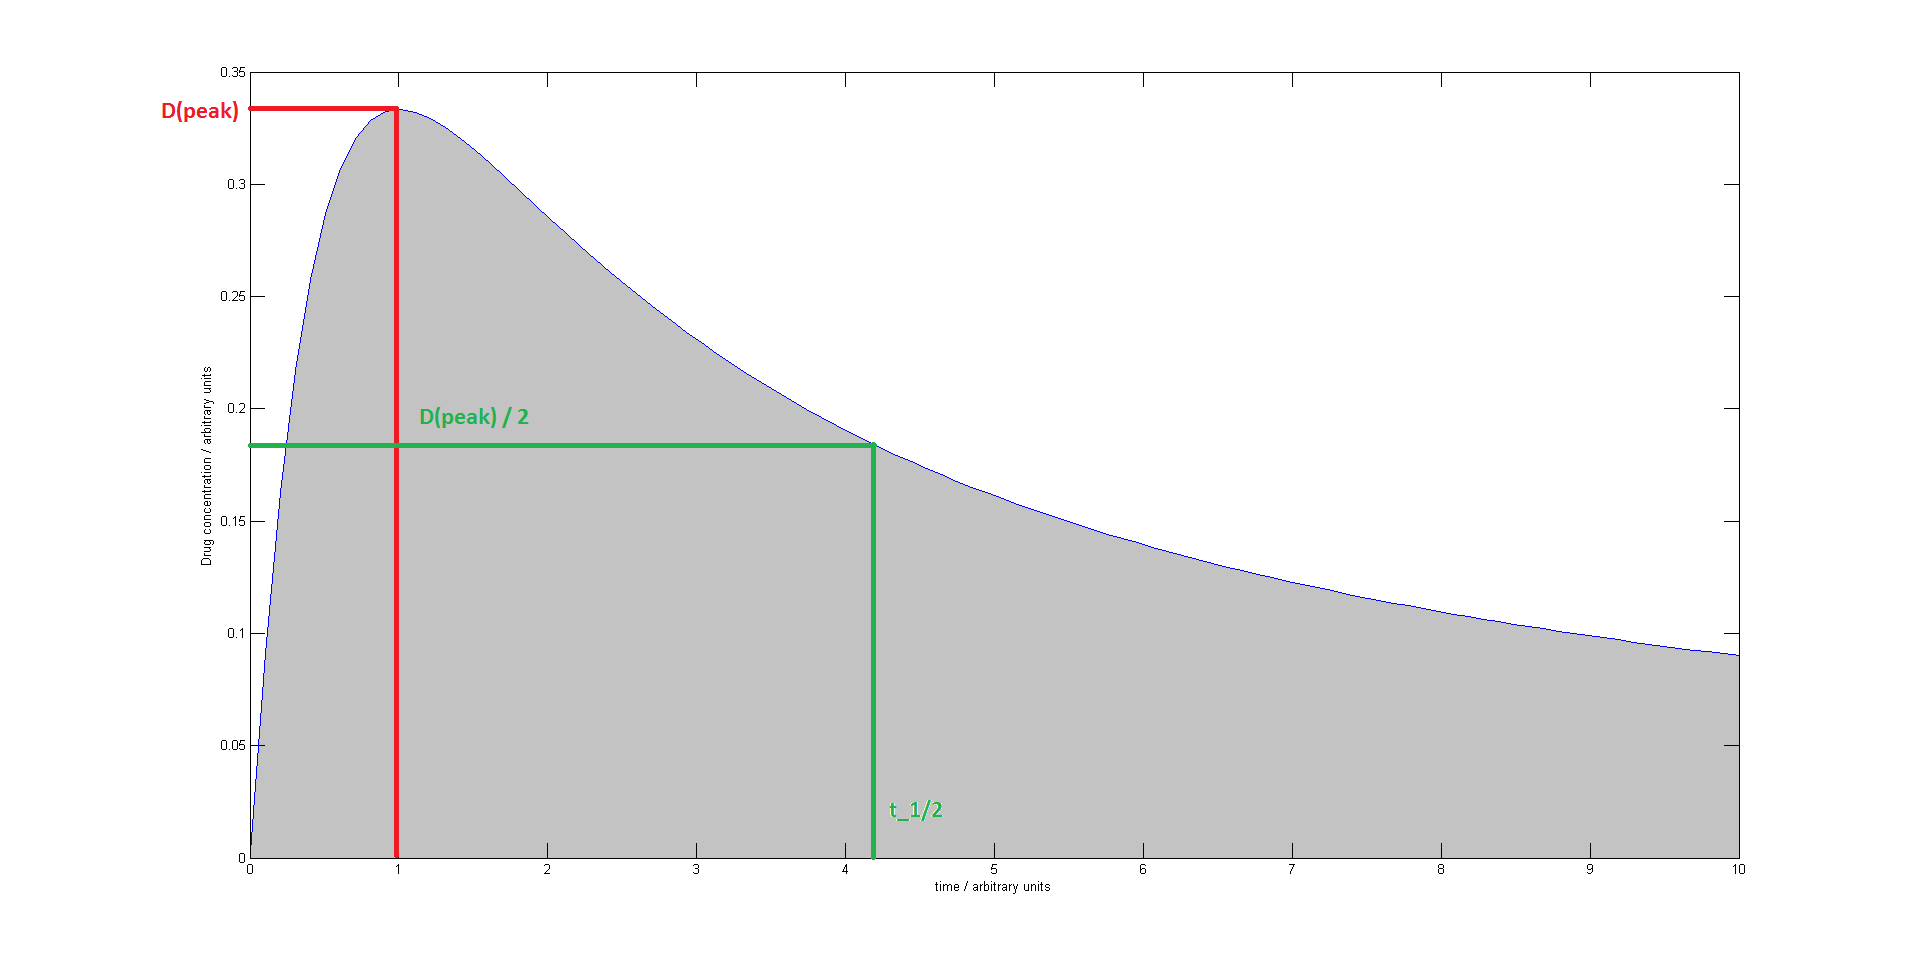
\includegraphics[width=150mm]{DrugProfile.png}
\caption{Plot of $\epsilon(t)$ against $t$ according to equation~\eqref{eq:drugeff}, for $c_1 = c_2 = c_3 = 1$.}
\label{fig:DrugProfile}
\end{centering}
\end{figure}

To achieve this, we used a time-dependent expression for $\epsilon$ of the form
\begin{equation}
\epsilon(t) = \frac{c_{1}t}{1 + c_{2}t+c_{3}^{2}t^{2}}. \label{eq:drugeff}
\end{equation}
Equation \eqref{eq:drugeff} seeks to emulate a realistic drug concentration profile in infected tissue.\footnote{An alternative approach we considered was to adopt a conventional 2-compartment pharmacokinetic model (see reference~\cite{Tsoukias} for an example), explicitly modelling drug concentrations as extra dynamic variables to be solved alongside the originals.}
A rapid initial surge in drug concentration following administration ($t = 0$), is followed by a slow, exponential purging of the drug from the tissues as it is excreted (figure~\ref{fig:DrugProfile}). The parameters in equation~\ref{eq:drugeff} can be found by fitting to known experimental data pertaining to the drug's pharmacokinetic profile.
% by Antonietta
Specifically, its peak time $t_{\textrm{peak}}$, when the full concentration $d_{\textrm{max}}$ of the drug has been released, and its half life $t_{\textrm{half}}$, which is the time after administration at which the concentration of the drug has reached half its maximal value. The constants $c_1$, $c_2$ and $c_3$ relate to the experimental data $d_{\textrm{max}}$, $t_{\textrm{peak}}$ and $t_{\textrm{half}}$ as follows:
\begin{eqnarray}
c_3 &=& \frac{1}{t_{\textrm{peak}}}\\
c_2 &=& \frac{(c_3 t_{\textrm{half}})^2 - 4 c_3 t_{\textrm{half}} + 1}{t_{\textrm{half}}}\\
c_1 &=& d_{\textrm{max}} (2 c_3 + c_2)
\end{eqnarray}
Also, in order to control the time of administration, a further parameter $t_{on}$ has to be introduced, and equation \eqref{eq:drugeff} changed to the form
\begin{equation}
\epsilon(n) = \left\{ 
   \begin{array}{l l}
     0 & \quad \text{for} \quad 0 \leq t \leq t_{on}\\
     \frac{\displaystyle c_{1}(t-t_{on})}{\displaystyle 1 + c_{2}(t-t_{on})+c_{3}^{2}(t-t_{on})^{2}} & \quad \text{for} \quad t > t_{on}
   \end{array} \right. \label{eq:drugadmin}
\end{equation}
\begin{figure}[htb]
\begin{centering}
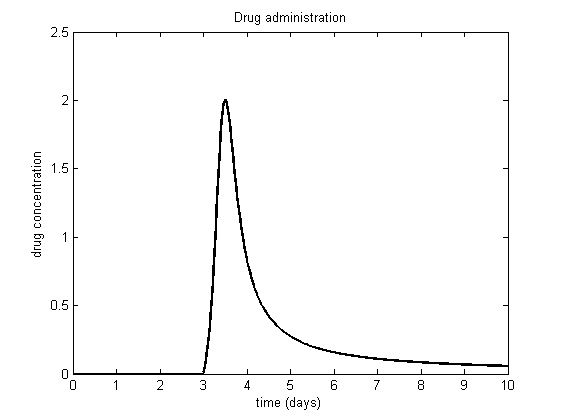
\includegraphics[width=150mm]{drugAdministration.png}
\caption{Plot of $\epsilon(t)$ against $t$ according to equation~\eqref{eq:drugadmin}. The input parameters for this graph are: $d_{max} = 2$, $t_{on} = 3$, $t_{peak} = 0.5$, $t_{half} = 0.9$, which results in $c_1 = 1.42$, $c_2 = -3.29$, $c_3 = 2$.}
\label{fig:DrugProfile}
\end{centering}
\end{figure}

Key questions include:
\begin{enumerate}
\item How does the time delay between infection onset and drug administration effect the treatment outcome?
\item Can polytherapy exhibit synergy? \textit{I.e.} could 2 drugs working together ever achieve more than the sum of their individual effects?
\end{enumerate}

\subsection{Effects of adding VNI antivirals -- some preliminary results}

Adding a drug variable of the form of equation~\eqref{eq:drugeff}  in the GUI of group G enabled us to probe the qualitative effects of the administration of a hypothetical VNI antiviral to an infected patient.\\

Firstly, we examined the effect of changing the drug dose (by changing the value of parameter $d_{\textrm{max}}$) on the viral population, as a function of time. Plotting the resulting curves of $V(t)$ against $t$ revealed some interesting behaviour (figure~\ref{fig:dosesweep}): as the drug dose was increased over the range $0.1 < d_{\textrm{max}} < 1$, the onset time of the ``viral surge'' observed by Hancioglu \textit{et al.}~\cite{Hancioglu} increased,\footnote{We note that the intial decline in severity with increasing dosage is actually followed by a marginal increase in same, for reasons as yet unknown to us.} accompanied by a marginal fall in severity as measured by the maximum of $V(t)$. Then, when the dosage exceeded a critcal value of around  $d_{\textrm{max}} = 0.52$, the viral surge peaks vanished, implying that there was sufficient drug present at the correct time so as to completely inhibit the viral take-over.\\
\begin{figure}[h!]
\begin{centering}
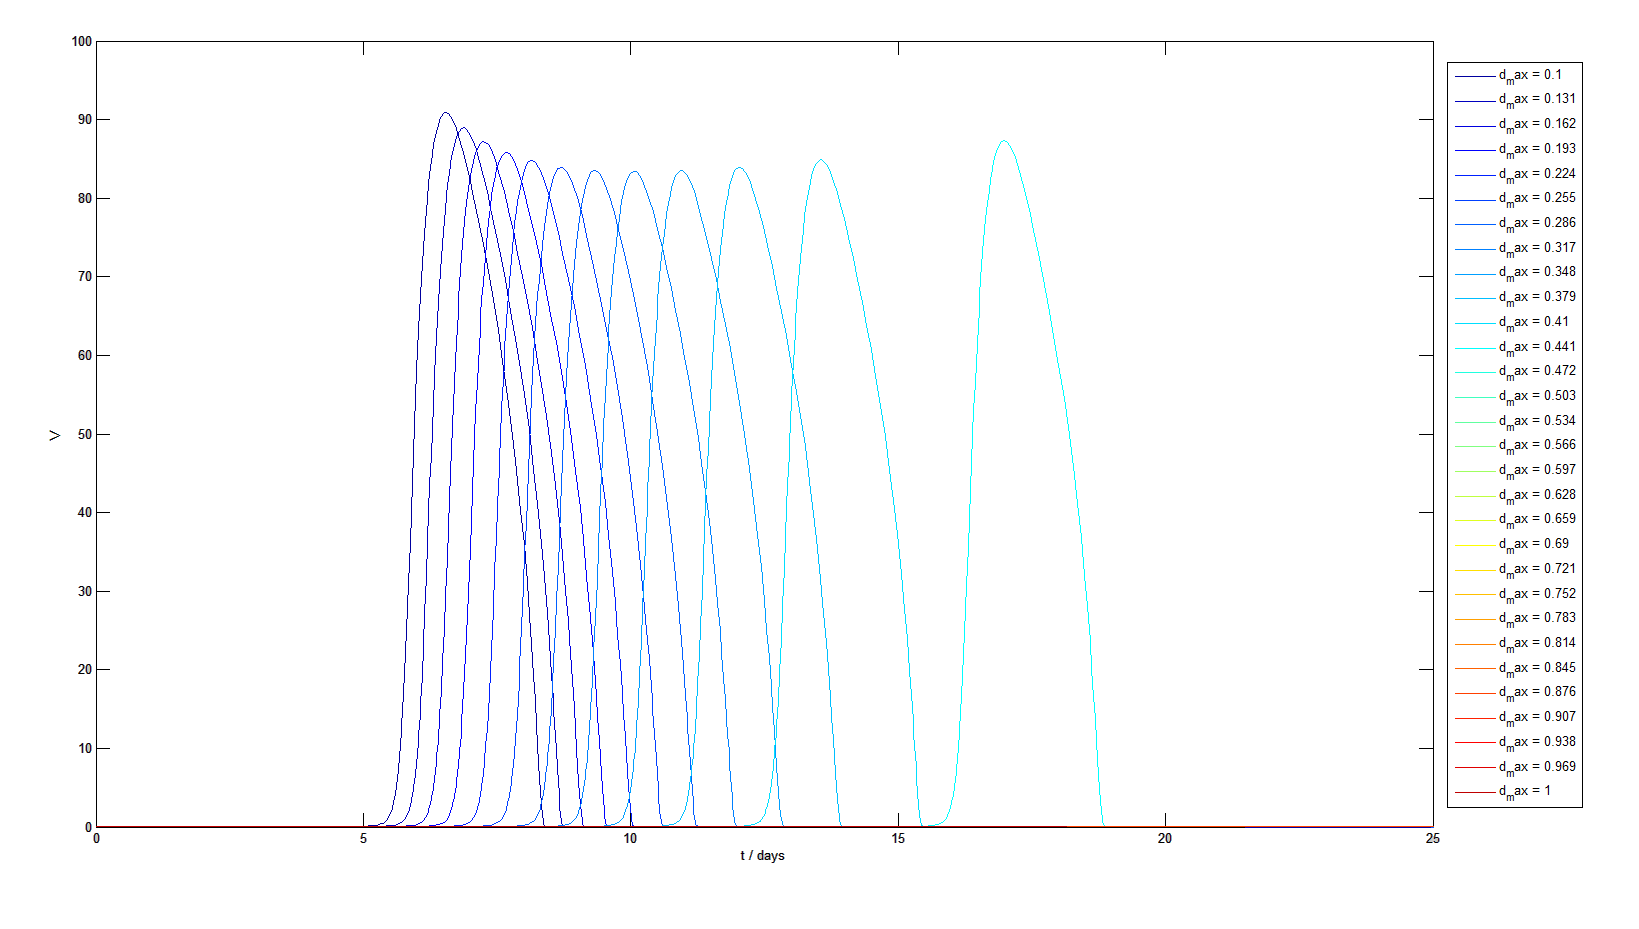
\includegraphics[width = \textwidth]{dosesweep.png}
\caption{Plot of viral population $V$ against $t$ for 30 values of $d_{\textrm{max}}$, given parameters $t_{\textrm{on}} = 0, t_{\textrm{peak}} = 3, t_{\textrm{half}} = 8$. The sudden disappearance of viral surges for $d \geq 0.543$ was unforseen.}
\label{fig:dosesweep}
\end{centering}
\end{figure}

Secondly, we investigated the effects of changing the time at which the drug was administered, for a fixed drug profile (figure~\ref{fig:timesweep}), using a parameter sweep extension to group G's GUI. We observed that the time of administration, $t_{\textrm{on}}$, was of critical importance in determining the severity of the infection. If drugs are administered too late after onset of an infection, then the drug is ineffective with respect to virus concentration, as should be expected. The only influence a late administration can have is on the speed of viral decrease.

\newpage
\begin{figure}[h!]
\begin{minipage}{0.5\textwidth}
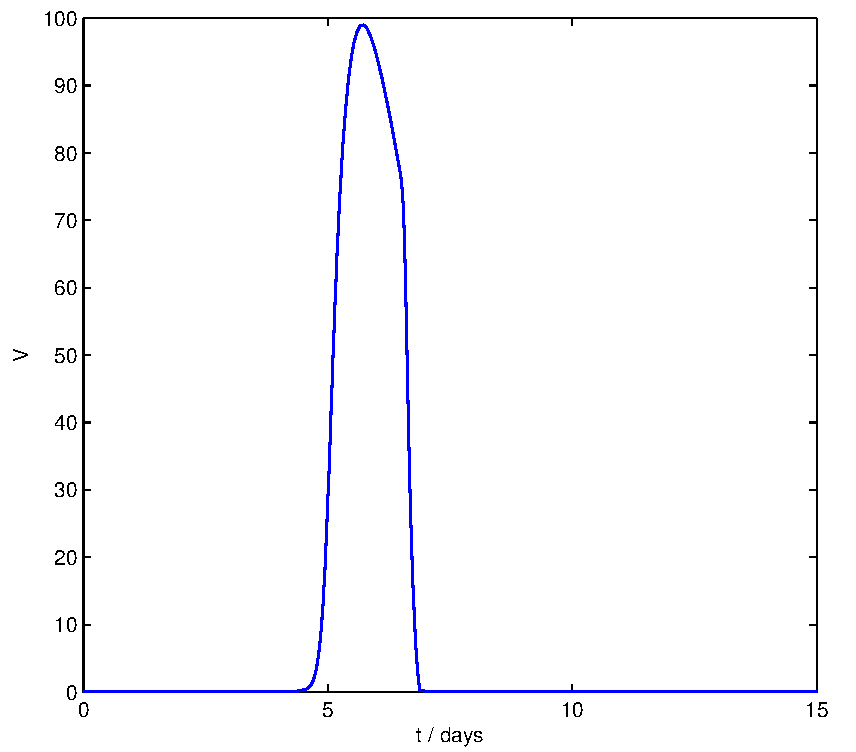
\includegraphics[height = 0.3\textheight]{drug_t0_6p5_scissored} %1
\end{minipage}
\begin{minipage}{0.5\textwidth}
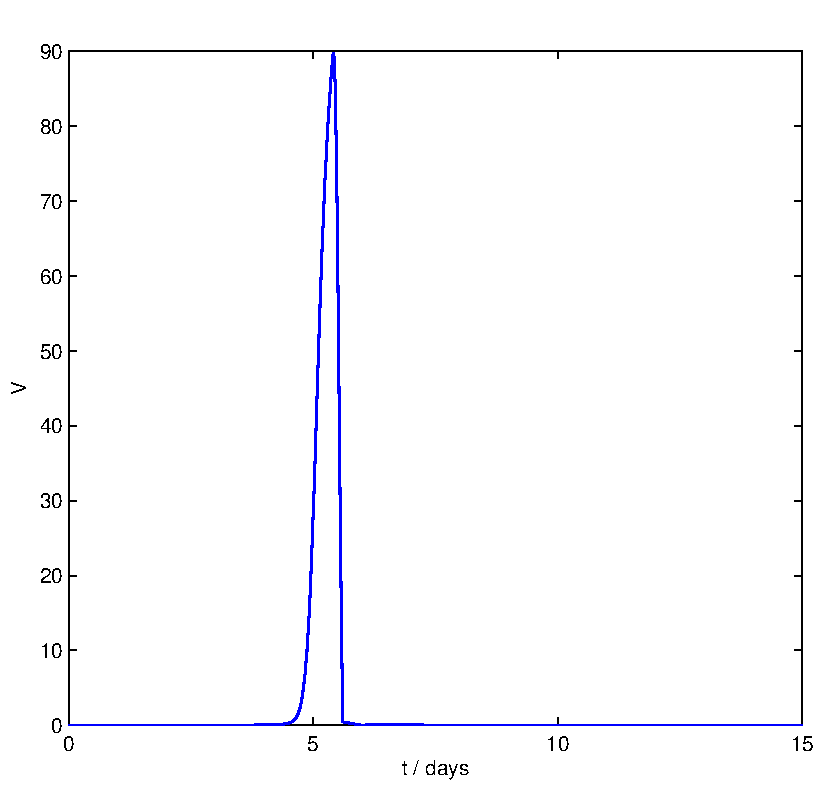
\includegraphics[height = 0.32\textheight]{drug_t0_5p4_scissored} %2
\end{minipage}

\begin{minipage}{0.5\textwidth}
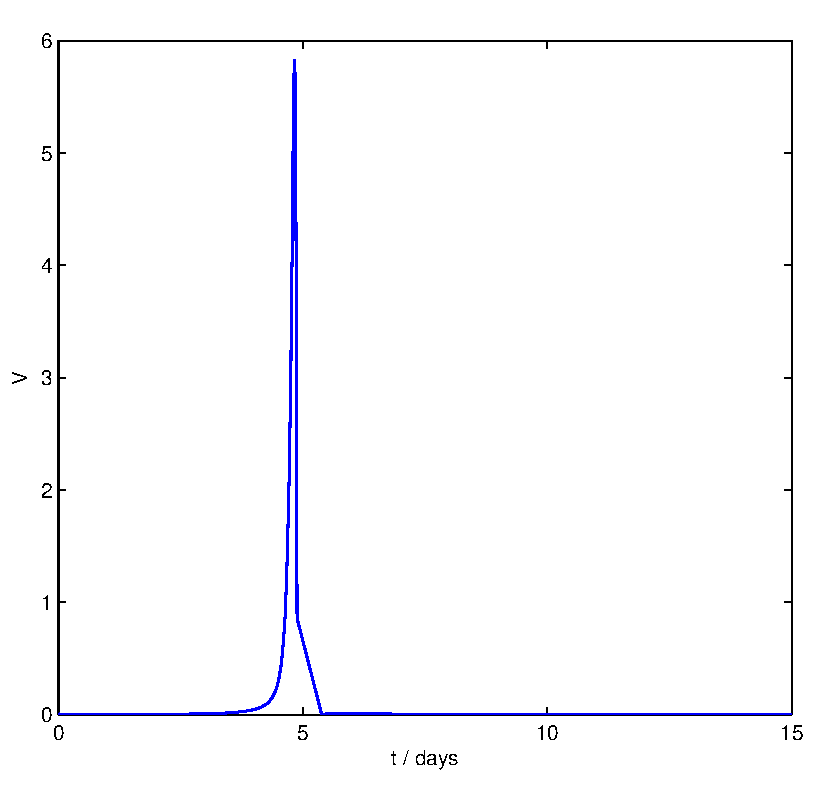
\includegraphics[height = 0.317\textheight]{drug_t0_4p8_scissored} %4
\end{minipage}
\begin{minipage}{0.5\textwidth}
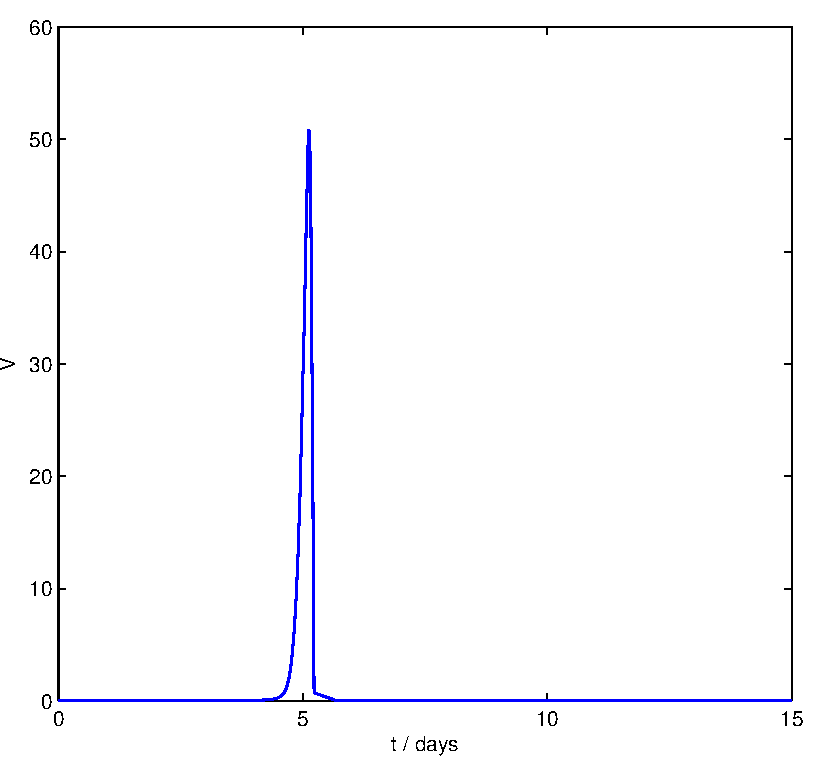
\includegraphics[height = 0.302\textheight]{drug_t0_5p1_scissored} %3
\end{minipage}
\caption{Consequences of altering the drug administration time for a given dose profile ( $d_{\textrm{max}} = 4, t_{\textrm{peak}} = 0.14, t_{\textrm{half}} = 0.33$ ). Clockwise from top left: $t_{\textrm{on}} = 6.5,~5.4,5.1,~4.8.$ Note the change in scale along the y axis -- administering the drug at times exactly coincidental with the viral surge can result in a 20-fold reduction in viral population.}
\label{fig:timesweep}
\end{figure}

We can infer from the parameter sweep shown in the previous plots, that the drug is most effective when administered around $t_{on} = 4.8$. We used this value of $t_{on}$ to check the effect of the maximum drug concentration $d_{max}$ on the virus concentration. We found that the concentration of viruses drop even for small values of $d_{max}$, but rises again if it has not reached a certain threshold, albeit not as high as without administering drugs.
\newpage

\begin{figure}[h!]
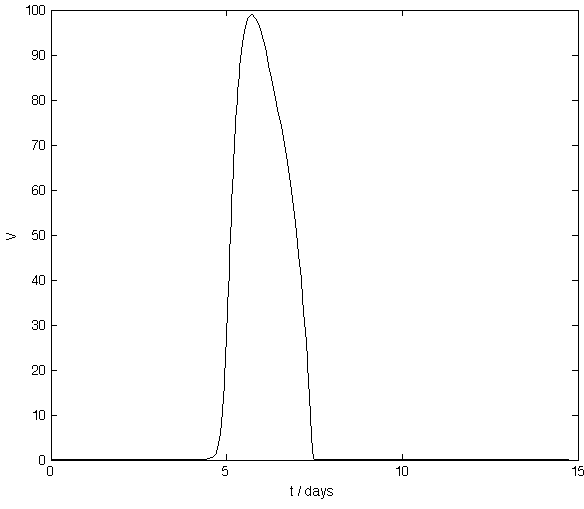
\includegraphics[width=75mm]{drug_zero.png}
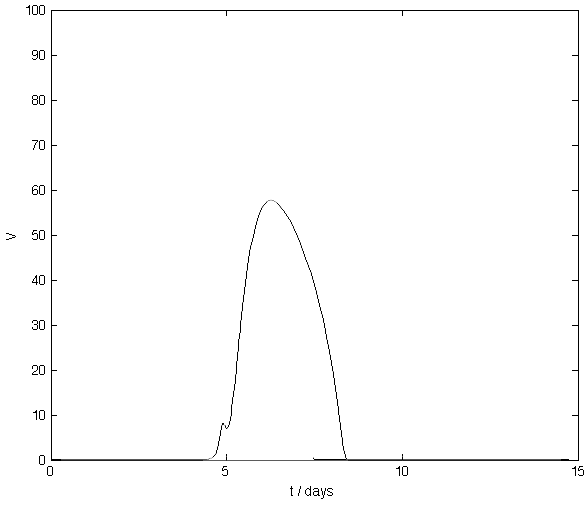
\includegraphics[width=75mm]{drug_one.png}
\newline
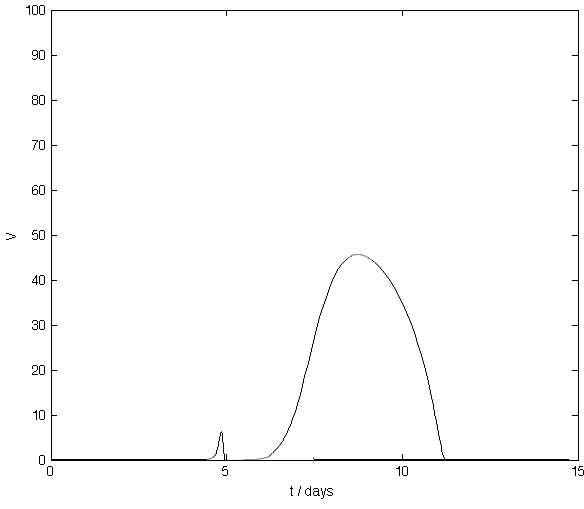
\includegraphics[width=75mm]{drug_two.png}
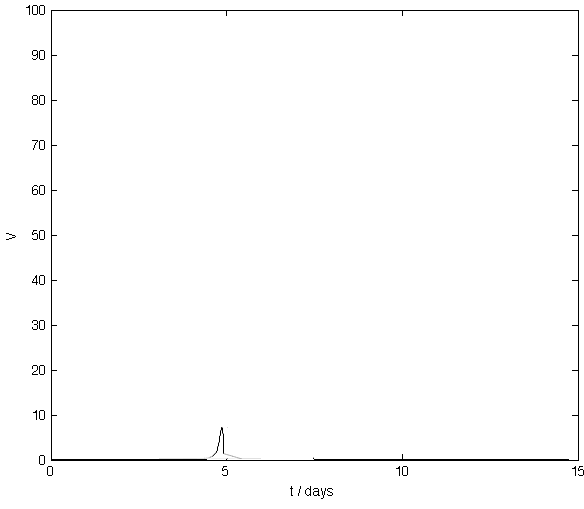
\includegraphics[width=75mm]{drug_three.png}
\caption{Plot of virus concentration versus time. The administration, peak and half-life times are held constant, just the maximum drug concentration is varied. The parameters are $t_{on} = 4.8$, $t_{peak} = 0.15$, $t_{half} = 0.4$, and $d_{max}$ varies in reading order from top left to bottom right through the values 0, 1, 2, 3. The maximum values of the virus concentrations drop from approx. 100, 60, 45 to 6 (again in reading order).}
\label{fig:onsetTimes}
\end{figure}

Generating representative plots of virus concentration versus time under drug administration poses the same problems as the original model. That is to say, that there is a far too large dependency on parameters that cannot (presently) be derived from experimental measurements. However, it is possible to infer certain dependencies on the parameters with the drug administration model as is.

\newpage
\section{ T\textsubscript{H} cells and Plasma Cell Dynamics} %By Jin
In the original model, the interaction of T\textsubscript{H}1 and T\textsubscript{H}2 cells were omitted with almost no justification - this seems unusual, especially considering how critical T\textsubscript{H} cells are fundamental to the clonal expansion of B-cells and their transition into plasma cells. Interestingly, new research suggests that it's neither T\textsubscript{H}1 or T\textsubscript{H}2 cells; instead, another cell type, the follicular helper T-cell, T\textsubscript{FH}, facilitates the switch ~\cite{Swain}. Though it would be ideal to integrate T\textsubscript{FH}:B-cell interaction into the model to enhance its biological relevance, their interaction has not yet been substantially modelled and our group felt it was precocious to propose an entirely new equation to model this interaction. On the other hand, the interaction of T-cells and B-cells has been modelled elsewhere ~\cite{Carneiro1}~\cite{Carneiro2}.\\ 

The change in T-cell population to antigen $k$ (\emph{i.e.} $\frac{dT_k}{dt}$) is dependent on the T-cell death rate ($k_{DT}$), proliferation rate ($k_{PT}$), thymic output rate ($k_{ST}$) and the function $\alpha{T}$ which depends on $\pi_{k}$ (stimulatory signal for T-cell activation), $\eta_{k}$ (inhibitory signal for T-cell activation), $T_{k}$, and two constants $a_{T1}$ and $a_{T2}$, hence leading to the equation:

\begin{eqnarray}
\frac{dT_k}{dt} &=& -k_{DT} \cdot T_k + k_{PT} \cdot \alpha_{T}(\pi_{k}, n_{k}, T_{k}) + k_{ST}; \label{dTK} \\
\alpha_{T}(\pi_{k}, \eta_{k}, T_{k}) &=& exp\left[-\left(\frac{log(\eta_{k}) - a_{T1}}{a_{T2}}\right)^{2}\right] \cdot \pi_{k} \cdot T_{k}
\end{eqnarray}

The population of active B cells, $B_{i}$, is dependent on the T-cell population; like equation ~\ref{dTK}, $B_{i}$ depends on B-cell death rate ($k_{DB}$), proliferation rate ($k_{PB}$), and the function $\alpha{B}$ (which depends on $\sigma_{i}$ [B cell induction signal], $\tau_{i}$ [number of active T cells], $\beta_{i}$ [the number of induced B cells] and $B_{i}$), thus leading to:
\begin{eqnarray}
\frac{dB_i}{dt} &=& -k_{DB} \cdot B_i + k_{PB} \cdot \alpha_{B}(\sigma_{i}, \tau_{i}, B_{i}); ~\label{dBI} \\
\alpha_{B}(\sigma_{i}, \tau_{i}, B_{i}) &=& \frac{\tau_{i}\cdot{\beta_{i}}}{\tau_{i} + \beta_{i}}, \\
\beta_{i} &=&  exp\left[-\left(\frac{log(\sigma_{i}) - b_{1}}{b_{2}}\right)^{2}\right] \cdot B_{i}
\end{eqnarray}

Surprisingly, for the purposes of analysis, the authors simplify both ~\ref{dTK} and ~\ref{dBI} assuming that there is at least one activated T-cell, thus reducing this system to:
\begin{eqnarray}
\frac{dT_k}{dt} &=& (k_{PT}-k_{DT}) \cdot T_k \\ ~\label{dTKSimple}
\frac{dB_i}{dt} &=& -k_{DB} \cdot B_i + k_{PB} \cdot \frac{T_{k} \cdot B_{i}}{T_{k}+B_{i}}; ~\label{dBISimple}
\end{eqnarray}

Given this new simplified formula, we decided to assimilate these two equations into the existing computational model. Unfortunately, one of the biggest challenges was actually fitting the newly-defined T\textsubscript{FH} cells into the overall scheme in Figure ~\ref{newmodel}. Considering that the mechanism of T\textsubscript{FH} cell differentiation remains undefined and the possibility that T\textsubscript{FH} cells are activated by B cells ~\cite{Crotty}, the equations that we are using may be inaccurate. On the other hand, there is sufficient evidence to suggest that T\textsubscript{FH} cells are activated by signals derived from APCs - thus, continuing with this notion, we suggest that equation ~\ref{dTKSimple} is scaled by the population of APCs, $M$.

\begin{equation}
\frac{dT_k}{dt} = (k_{PT}-k_{DT}) \cdot T_k \cdot M \\
\end{equation}

Under the new scheme, na\"\i ve B-cell activation by T\textsubscript{FH} cells can be represented by equation ~\ref{dBISimple}. As for the subsequent formation of plasma cells from B cells, we can see the original ODE for the formation of plasma cells (where $b_{PM}$ and $\alpha{P}$ are constants representing plasma cell synthesis and death, respectively):
\begin{equation}
\frac{dP}{dt} = b_{PM}MP + \alpha_{P}(1 - P)
\end{equation}

We decided to modify this equation slightly; we retained the constants as they represent properties intrinsic to the \emph{plasma cell}. However, we changed the dependence of plasma cell synthesis to the population of active B cells, $B_{i}$, rather than M (\emph{N.B. }To avoid confusion in nomenclature, $b_{PM}$ was renamed to $b_{PB}$). Therefore, we would attain:
\begin{equation}
\frac{dP}{dt} = b_{PB}B_{i}P + \alpha_{P}(1 - P)
\end{equation}

In summary, to account for the role of helper T cells in plasma cell synthesis with the influenza virus (V) as the antigen, we propose the following system of ODEs:
\begin{eqnarray*}
\frac{dT_V}{dt} &=& (k_{PT}-k_{DT}) \cdot T_V \cdot M \\
\frac{dB_i}{dt} &=& -k_{DB} \cdot B_i + k_{PB} \cdot \frac{T_{V} \cdot B_{i}}{T_{V}+B_{i}} \\
\frac{dP}{dt} &=& b_{PB}B_{i}P + \alpha_{P}(1 - P)
\end{eqnarray*}

Due to the addition of these new compartments, the inherited C++ mex function and its header, \texttt{mexodestiff.cpp} and \texttt{mexodestiff.hpp}, were re-adjusted. Much of the code was retained, with the exception that new variables were defined as necessary, and the Jacobian matrix in the header file was re-defined to accommodate for the two new compartments.

\section{Introduction of Stochasticity} %Done by Jin and Owen
To improve the current computational model, we felt that giving the user the freedom to incorporate stochasticity into their analyses was essential. The idea was not to replace the code, but instead give the user a more realistic account of how cell populations and viral titre can vary over time. We decided that the two areas in which introduction of stochasticity were most biologiclaly justified were in virus production and development of antibody affinity. It is understood that there is a wide range of variability in virus production from infected cells \cite{MitchellJanuary152011}, so we felt justified in adding a noise term which affects the total virus population V.\\

Similarly, the model already incorporates the affinity maturation of antibodies, but fails to model the fundamentally stochastic nature of the recombination process. In theory, every antibody is constructed from a diverse genetic framework and every antibody has a different affinity for the virus - only the antibody that binds strongest is selected for further expansion in the geminal centres \cite{Grimaldi15022005}. Consequently, we felt that another target for noise terms was the rate of change of variable S, in order to incorporate the iterative, random process of antibody selection.\\

There were two possible ways of approaching this problem; it is possible to introduce stochastic noise into either the cell populations or the dynamical rate paramters. Both were explored, and are discussed below.

\subsection{Stochastic Populations}

The study of stochastic differential equations (SDEs) is a widely studied topics in mathematics, with many resources for different algorithms and implementations \cite{2001}. The ideal is to solve a differential equation with a well-defined noise function adding a stochastic element over time:

\begin{align}
\frac{\mathrm d X}{\mathrm d t}(t) = \mathrm f (X) + \text{``noise''}
\end{align}

In the above, $f(X,t)$ is the ``drift function" of the system that would comprise a traditional ODE and ``noise'' is the component that contributes the stochastic element with time. It is possible to introduce a traditional finite-difference forward-regression approach, by implementing the Euler-Maruyama method for an SDE, such that:

\begin{align}
\label{eqn:eulerMaruyama}
X(t+\delta t) = X(t) + (\delta t)\, \mathrm f (X(t)) + \sqrt{ \delta t}\, \mathrm G (X(t))\, \eta \quad \text{such that} \quad \eta \in N(0,1)
\end{align}

Here, $N(0,1)$ is a normal distribution, with a mean of zero and standard deviation of one and $G(X(t))$ is the ``diffusion coefficient'' for our system. Given access to the functions $f(x)$ and $G(X)$ and a normally distributed random number generator, it is possible to solve this iteratively, with each new timestep explicitly using the previous one. This is a simple but reliable implementation, which represents a good method for introducing background noise into the concentrations of variables in our system.

\subsection{Stochastic Rates}

The next approach, which is possibly more theoretically justifiable, is to allow the parameters of the ODE system to vary stochastically with each call of the function $f(X(T))$. This allows the code to isolate the mechanisms are contributing noise, rather than simply adding some arbitrary amount of stochasticity to the variable after each timestep. This method allows for the standard library of ODE solving regression algorithms, since it is the drift function that contributes noise rather than the finite different method itself. It is consequently slightly easier to implement in various languages.

\subsection{Implementation in Matlab\textsuperscript{\textregistered}}

These two approaches were implemented in two different solver functions: \texttt{sdesolver()} and \texttt{sderatesolver()}, respectively. These resembled the native Matlab\textsuperscript{\textregistered} solvers, but with an extra input, describing the nature of the diffusion coefficient $G(X(t))$. \texttt{sdesolver()} is handed a two by ten dimensional matrix containing the vectors $a$ and $b$, used such that $G(X)=a.$*$X.^b$, elementwise. This gives a wide sampling of potential diffusion functions, allowing for easy sampling of interesting parameter spaces. The second function, \texttt{sderatesolver()}, demands two inputs, which specify the strength of the noise added to the creation rates of V and S, these being judged to be the processes most likely to realistically exhibit highly stochastic behaviour. A difficulty of implementation involved forcing all variables to remain non--negative: if either the numerical methods or stochastic noise push any variables below zero into an unphysical region of phase space, the variables would quickly and collectively diverge into positives or negative infinities. This was avoided with a simple zero check and modification.

\subsection{Implementation in C with Mex files} %Written by Malte
The implementation of stochasticity in C was done reusing parts of Group G's C++ mex code and converting this to C syntax and adding a stochastic ODE solver after the Euler-Maruyama method described earlier. A 10 by 2 matrix with noise parameters a and b, representing the inputs in $G(x) = ax^b$ as described in the section above, was read in and used to calculate a noise factor, $G(x)$ from equation \eqref{eqn:eulerMaruyama}. In order to generate a Gaussian random variable, denoted $\eta$ in the aforementioned equation, a Box-Mueller transform \cite{box1958} was used:

\begin{align}
\label{eqn:boxMueller}
X_1 = \sqrt{ -2\, \log(U_1)}\, \cos(2 \pi U_2) 
\end{align}

In this equation $U_1$ and $U_2$ denote uniformly distributed random numbers in the interval $[0;1]$. The method used to create these uniformly distributed random numbers was: 

$\textit{rand()}\,\%\, 1001 / 1000$ 
The random number generator \textit{rand()} was seeded by the CPU time at every loop iteration, thus the same seed was used for the $2N$ calls to \textit{rand()} at every iteration, where $N$ is the number of equations in the system of coupled ODEs. This seeding method can be a cause for systematic error, due ot the pseudo-randomness of the \textit{rand()} function in C. A further cause of systematic error is if RAND\_MAX $\gg 1000$ is not true. In this case there is a bias towards lower values. Furthermore, the uniform random variable only being sampled to 3 decimal places can cause errors in the distribution of the gaussian random variable.\\

The mex function was tested against the same code in matlab for different numbers of iterations of the main loop, dependent on start and end times and the timestep. The time comparison obtained from this can be seen in Table \ref{tbl:matlabCComparison}.

\begin{table}
\centering
\begin{tabular}{ | c | c | c | c | }
\hline
Iteration & Matlab Code Time (s) & Mex Code Time (s) & Speed up factor \\ \hline
1000 & 0.0016 & 0.0516 & 32.25 \\ \hline
3000 & 0.0045 & 0.1550 & 34.44 \\ \hline
10000 & 0.0147 & 0.5130 & 34.90 \\ \hline
100000 & 0.1480 & 5.1298 & 34.66 \\
\hline
\end{tabular}
\caption{Comparison of Run times for Matlab and C implementation of the stochastic solver. The simulation end time was varied from 10 to 1000 with start time 0 and timestep 0.01. All other parameters used were given by the default values in the GUI.}
\label{tbl:matlabCComparison}
\end{table}

The mex solver in C exhibits some numerical instability, which occurs occasionally when the initial value for the Virus population, $V$, is at around 0.01 and the timestep is of a similar order of magnitude. This is an instability which is inherent in the method and its removal is out of the scope of this project. \\

Upon confirmation of the efficiency of the mex solver, this was then re-designed with the two additional compartments to generate a 12 by 2 matrix with appropriate noise parameters.

\section{Results}

We observed several interesting phenomena over the course of exploring parameter and solver configurations for the SDEs. These can be loosely grouped into two classes, those of noise propagation and virus resurgence.

\subsection{Noise propagation}

An interesting question which we addressed is the extent to which noise introduced to one parameter will appear in the output of another parameter. Choosing S and V as being test cases, we added noise to each independently and both together, observing the extent to which this effect the behaviour of other variables. We found that noise added to V became manifest in slight perturbations to the response curves of H, I and M., although the curves were still qualitatively the same objects. Noise added to the variable S had no obvious effect: despite being relatively well--connected in the system of ODEs, the other variables were less effected by perturbations in S. This may be owing to the role of S as a logical variable, ranging from its steady states at zero and one; stochastic variation of this variable may be insignificant compared to the overall logical state of the efficacy.

\subsection{Virus Resurgence}

One dynamically significant effect of adding noise to either the virus population V or the rate of creation of V by infected cells is the occurrence of virus resurgence and infection. If the noise introduced to the rate of creation of V is significantly large then the virus population plotted against time will feature more than one spike, representing a reappearance of the virus population in the cell population. We speculate that this is the stochasticity pushing the depleted virus count above a threshold, sparking another wave of infection when the antibody count has decayed sufficiently. This new wave is accompanied by a corresponding rise in antibodies in response, hoping to combat the infection. It is interesting that the subsequent virus and antibody peaks are significantly lower than those of the first wave: this can be explained by reference to the antibody efficacy S. This grows every time a new infection appears, describing the cell population's capacity to ``remember'' how to combat the virus, making the virus less successful and demanding less antibody concentration for each wave. These effects can be observed in Figure \ref{resurgance}.

\begin{figure}
\begin{center}
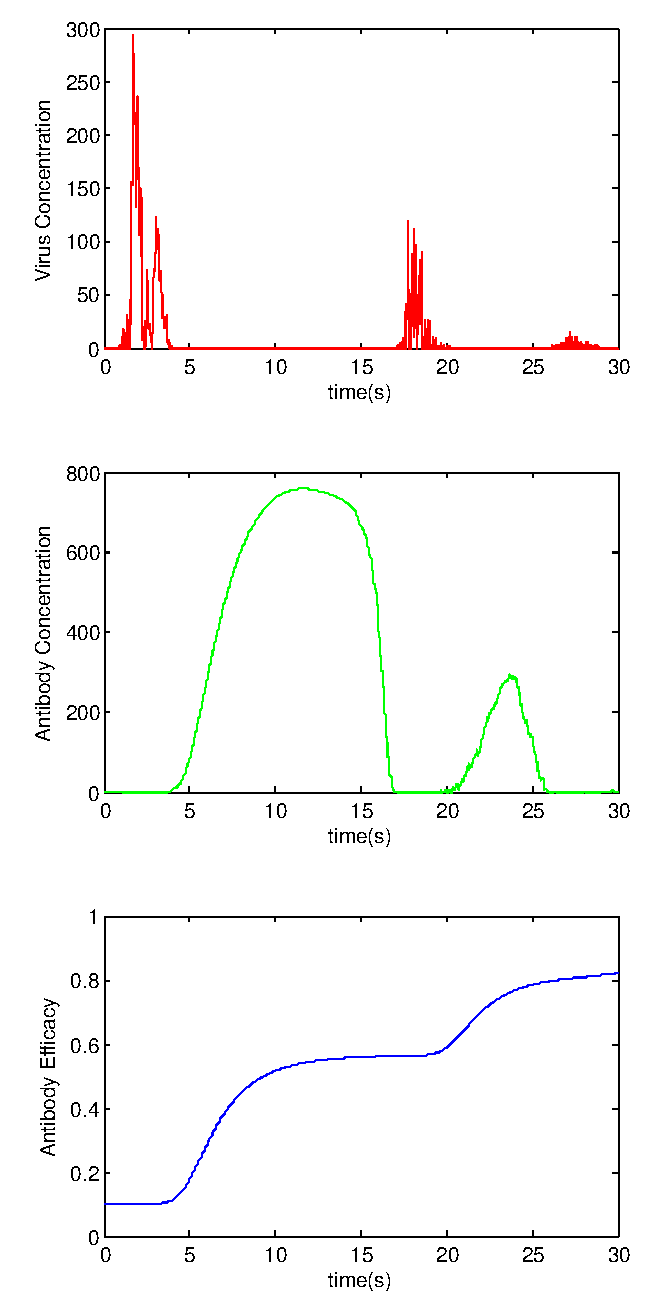
\includegraphics[width=120mm]{Resurgance_scissored.pdf}
\label{resurgance}
\caption{Outputs for V, A and S against time, using the default GUI parameter set and \texttt{sderatesolver()}, with \texttt{NoiseParameters.VNoise = 5} and \texttt{NoiseParameters.SNoise=0}}
\end{center}
\end{figure}

%\chapter{Appendix}

\bibliography{GroupDReportBibTex}
\bibliographystyle{plain}

\end{document}